\documentclass{article}
\usepackage{ctex}
\title{编译原理 作业8}
\author{} 
\date{}
\usepackage[a4paper,left=10mm,right=10mm,top=15mm,bottom=15mm]{geometry} 
\usepackage{graphicx} 
\usepackage{makecell}
\usepackage[linguistics]{forest}
\usepackage{amsmath}

\begin{document}

\textbf{9.4.}第一次进入F后, 运行栈的内容:

\begin{tabbing}
    \hspace{1.5cm} \= \hspace{1.5cm} \= \hspace{1.5cm} \= \kill
    \> 10 \> 4\\

    \> 9 \> 0\\

    \> 8 \> n(形参)\\

    \> 7 \> 1(形参个数)\\

    \> 6 \> 2(全局display)\\

    \> 5 \> 返回地址\\

    \> 4 \> 0 \\

    \> 3 \> k\\

    \> 2 \> 0(display)\\

    \> 1 \> 返回地址\\

    \> 0 \> 0\\
\end{tabbing}

第二次进入F后, display的内容为:

\begin{tabbing}
    \hspace{1.5cm} \= \hspace{1.5cm} \= \kill
    \> 11 \\

    \> 0 \\
\end{tabbing}

第二次进入F后, 运行栈的内容:

\begin{tabbing}
    \hspace{1.5cm} \= \hspace{1.5cm} \= \hspace{1.5cm} \= \kill
    \> 17 \> 11\\

    \> 16 \> 0\\

    \> 15 \> n(形参)\\

    \> 14 \> 1(形参个数)\\

    \> 13 \> 9(全局display)\\

    \> 12 \> 返回地址\\

    \> 11 \> 4\\

    \> 10 \> 4\\

    \> 9 \> 0\\

    \> 8 \> n(形参)\\

    \> 7 \> 1(形参个数)\\

    \> 6 \> 2(全局display)\\

    \> 5 \> 返回地址\\

    \> 4 \> 0 \\

    \> 3 \> k\\

    \> 2 \> 0(display)\\

    \> 1 \> 返回地址\\

    \> 0 \> 0\\
\end{tabbing}

\textbf{9.5.}运行到(1)时的运行栈:(静态链)

\begin{tabbing}
    \hspace{1.5cm} \= \hspace{1.5cm} \= \hspace{1.5cm} \= \kill

    \>15 \> c\\

    \>14 \> 0(形参个数)\\

    \>13 \> 5\\

    \>12 \> 返回地址\\

    \>11 \> 5\\

    \>10 \> p\\

    \>9 \> k(形参)\\

    \>8 \> 1(形参个数)\\

    \>7 \> 0\\

    \>6 \> 返回地址\\

    \>5 \> 0\\

    \>4 \> d \\

    \>3 \> i\\

    \>2 \> 0\\

    \>1 \> 返回地址\\

    \>0 \> 0\\

\end{tabbing}

运行到(2)时的运行栈:(静态链)

\begin{tabbing}
    \hspace{1.5cm} \= \hspace{1.5cm} \= \hspace{1.5cm} \= \kill
    \>15 \> c\\

    \>14 \> 0(形参个数)\\

    \>13 \> 5\\

    \>12 \> 返回地址\\

    \>11 \> 5\\

    \>10 \> p\\

    \>9 \> k(形参)\\

    \>8 \> 1(形参个数)\\

    \>7 \> 0\\

    \>6 \> 返回地址\\

    \>5 \> 0\\

    \>4 \> d \\

    \>3 \> i\\

    \>2 \> 0\\

    \>1 \> 返回地址\\

    \>0 \> 0\\

\end{tabbing}

运行到(1)时的运行栈:(display表)

\begin{tabbing}
    \hspace{1.5cm} \= \hspace{1.5cm} \= \hspace{1.5cm} \= \kill
    \>20 \> c\\

    \>19 \> 13\\

    \>18 \> 5\\

    \>17 \> 0\\

    \>16 \> 0(形参个数)\\

    \>15 \> 10(全局display)\\

    \>14 \> 返回地址\\

    \>13 \> 5\\

    \>12 \> p\\

    \>11 \> 5\\

    \>10 \> 0\\

    \>9 \> k(形参)\\

    \>8 \> 1(形参个数)\\

    \>7 \> 2(全局display)\\

    \>6 \> 返回地址\\

    \>5 \> 0\\

    \>4 \> d \\

    \>3 \> i\\

    \>2 \> 0(display)\\

    \>1 \> 返回地址\\

    \>0 \> 0\\

\end{tabbing}

运行到(2)时的运行栈:(display表)

\begin{tabbing}
    \hspace{1.5cm} \= \hspace{1.5cm} \= \hspace{1.5cm} \= \kill
    \>20 \> c\\

    \>19 \> 13\\

    \>18 \> 5\\

    \>17 \> 0\\

    \>16 \> 0(形参个数)\\

    \>15 \> 10(全局display)\\

    \>14 \> 返回地址\\

    \>13 \> 5\\

    \>12 \> p\\

    \>11 \> 5\\

    \>10 \> 0\\

    \>9 \> k(形参)\\

    \>8 \> 1(形参个数)\\

    \>7 \> 2(全局display)\\

    \>6 \> 返回地址\\

    \>5 \> 0\\

    \>4 \> d \\

    \>3 \> i\\

    \>2 \> 0(display)\\

    \>1 \> 返回地址\\

    \>0 \> 0\\

\end{tabbing}

\textbf{9.6.}
运行到标号10时运行栈的内容:

\begin{tabbing}
    \hspace{1.5cm} \= \hspace{1.5cm} \= \hspace{1.5cm} \= \kill
    \>24 \> g\\

\>23 \> f\\

\>22 \> 16\\

\>21 \> 6\\

\>20 \> 0\\

\>19 \> 0(形参个数)\\

\>18 \> 12(全局display)\\

\>17 \> 返回地址\\

\>16 \> 6\\

\>15 \> e\\

\>14 \> d\\

\>13 \> 6\\

\>12 \> 0\\

\>11 \> j\\

\>10 \> i\\

\>9 \> 2(形参个数)\\

\>8 \> 2(全局display)\\

\>7 \> 返回地址\\

\>6 \> 0\\

\>5 \> c\\

\>4 \> b\\

\>3 \> a\\

\>2 \> 0(display)\\

\>1 \> 返回地址\\

\>0 \> 0\\

\end{tabbing}

运行到标号11时运行栈的内容:

\begin{tabbing}
    \hspace{1.5cm} \= \hspace{1.5cm} \= \hspace{1.5cm} \= \kill
    \>26 \> j\\

    \>25 \> i\\


    \>24 \> h\\

    \>23 \> 16\\

    \>22 \> 6\\

    \>21 \> 0\\

    \>20 \> k\\

    \>19 \> 1(形参个数)\\

    \>18 \> 12(全局display)\\

    \>17 \> 返回地址\\

    \>16 \> 6\\

    \>15 \> e\\

\>14 \> d\\

\>13 \> 6\\

\>12 \> 0\\

\>11 \> j\\

\>10 \> i\\

\>9 \> 2(形参个数)\\

\>8 \> 2(全局display)\\

\>7 \> 返回地址\\

\>6 \> 0\\

\>5 \> c\\

\>4 \> b\\

\>3 \> a\\

\>2 \> 0(display)\\

\>1 \> 返回地址\\

\>0 \> 0\\

\end{tabbing}

\textbf{9.9.}

\textbf{(1)传名}

当过程被调用时,将被调用段的过程体复制到调用出现处,但必须将其中出现的任意形式参数都代之以相应的实参.
\begin{verbatim}
    A:=2;                                  
    B:=3;                                
    A:=A+1;                             
    A:=A+(A+B);                    
    print A;   
    A=9  
\end{verbatim}

\textbf{(2)传地址}

当程序控制转入被调用段后,被调用段首先把实参复制进相应的形式参数的形式单元中,过程体对形参的任何引用或赋值都被处理成对形式单元的间接访问.

当被调用段工作完毕返回时,形式单元(都是指示器)所指的实参单元就持有所希望的值.

\begin{verbatim}
    1)A:=2;B:=3;T:=A+B
    2)把T,A,A的地址复制进已知单元J1,J2,J3
    3)x:=J1;y:=J2;z:=J3       //把实参地址复制进形式单元,且J2=J3
    4)Y↑:=y↑+1
    Z↑:=z↑+x↑              // Y↑:对y的间接访问
                                Z↑:对z的间接访问
    5)print A
    A=8
\end{verbatim}

\textbf{(3)得到结果}

每个形参均对应两个单元,第一个存放实参地址,第二个存放实参值,在过程体中对形参的任何引用或赋值都看成是对它的第二个单元的直接访问,但在过程工作完毕返回前必须把第二个单元的内容放到第一个单元所指的那个实参单元中.
\begin{verbatim}
    1)A:=2;B:=3;T:=A+B
    2)把T,A,A的地址复制进已知单元J1,J2,J3
    3)x1:=J1;x2:=T;
    y1:=J2;y2:=A;
    z1:=J3;z2:=A;              //将实参的地址和值分别放进两个形式单元中
    4)y2:=y2+1; z2:=z2+x2;       //对形参第二个单元的直接访问
    5)x1↑:=x2; y1↑:=y2; z1↑:=z2   //返回前把第二个单元的内容存放到第一个单元所指的实参地址中
    6)print A
    A=7
\end{verbatim}

\textbf{(4)传值}

即被调用段开始工作时,首先把实参的值写进相应的形参单元中,然后就像使用局部变量一样使用这些形式单元.
\begin{verbatim}
    A:=2;
    B:=3;
    x:=A+B
    y:=A
    z:=A
    y:=y+1
    z:=z+x
    print A
    A=2
\end{verbatim}

过程调用不改变A的值.


\textbf{10.2.}
\begin{verbatim}
    read A, B
    F := 1
    C := A*A
    D := B*B
    if C < D 
        goto L1
    E := A*A
    F := F+1
    E := E+F
    write E
    halt
    L1:E := B*B
    F := F+2
    E := E+F
    write E
    if E>100 
        goto L2
    halt
    L2:F := F+1
    goto L1
\end{verbatim}
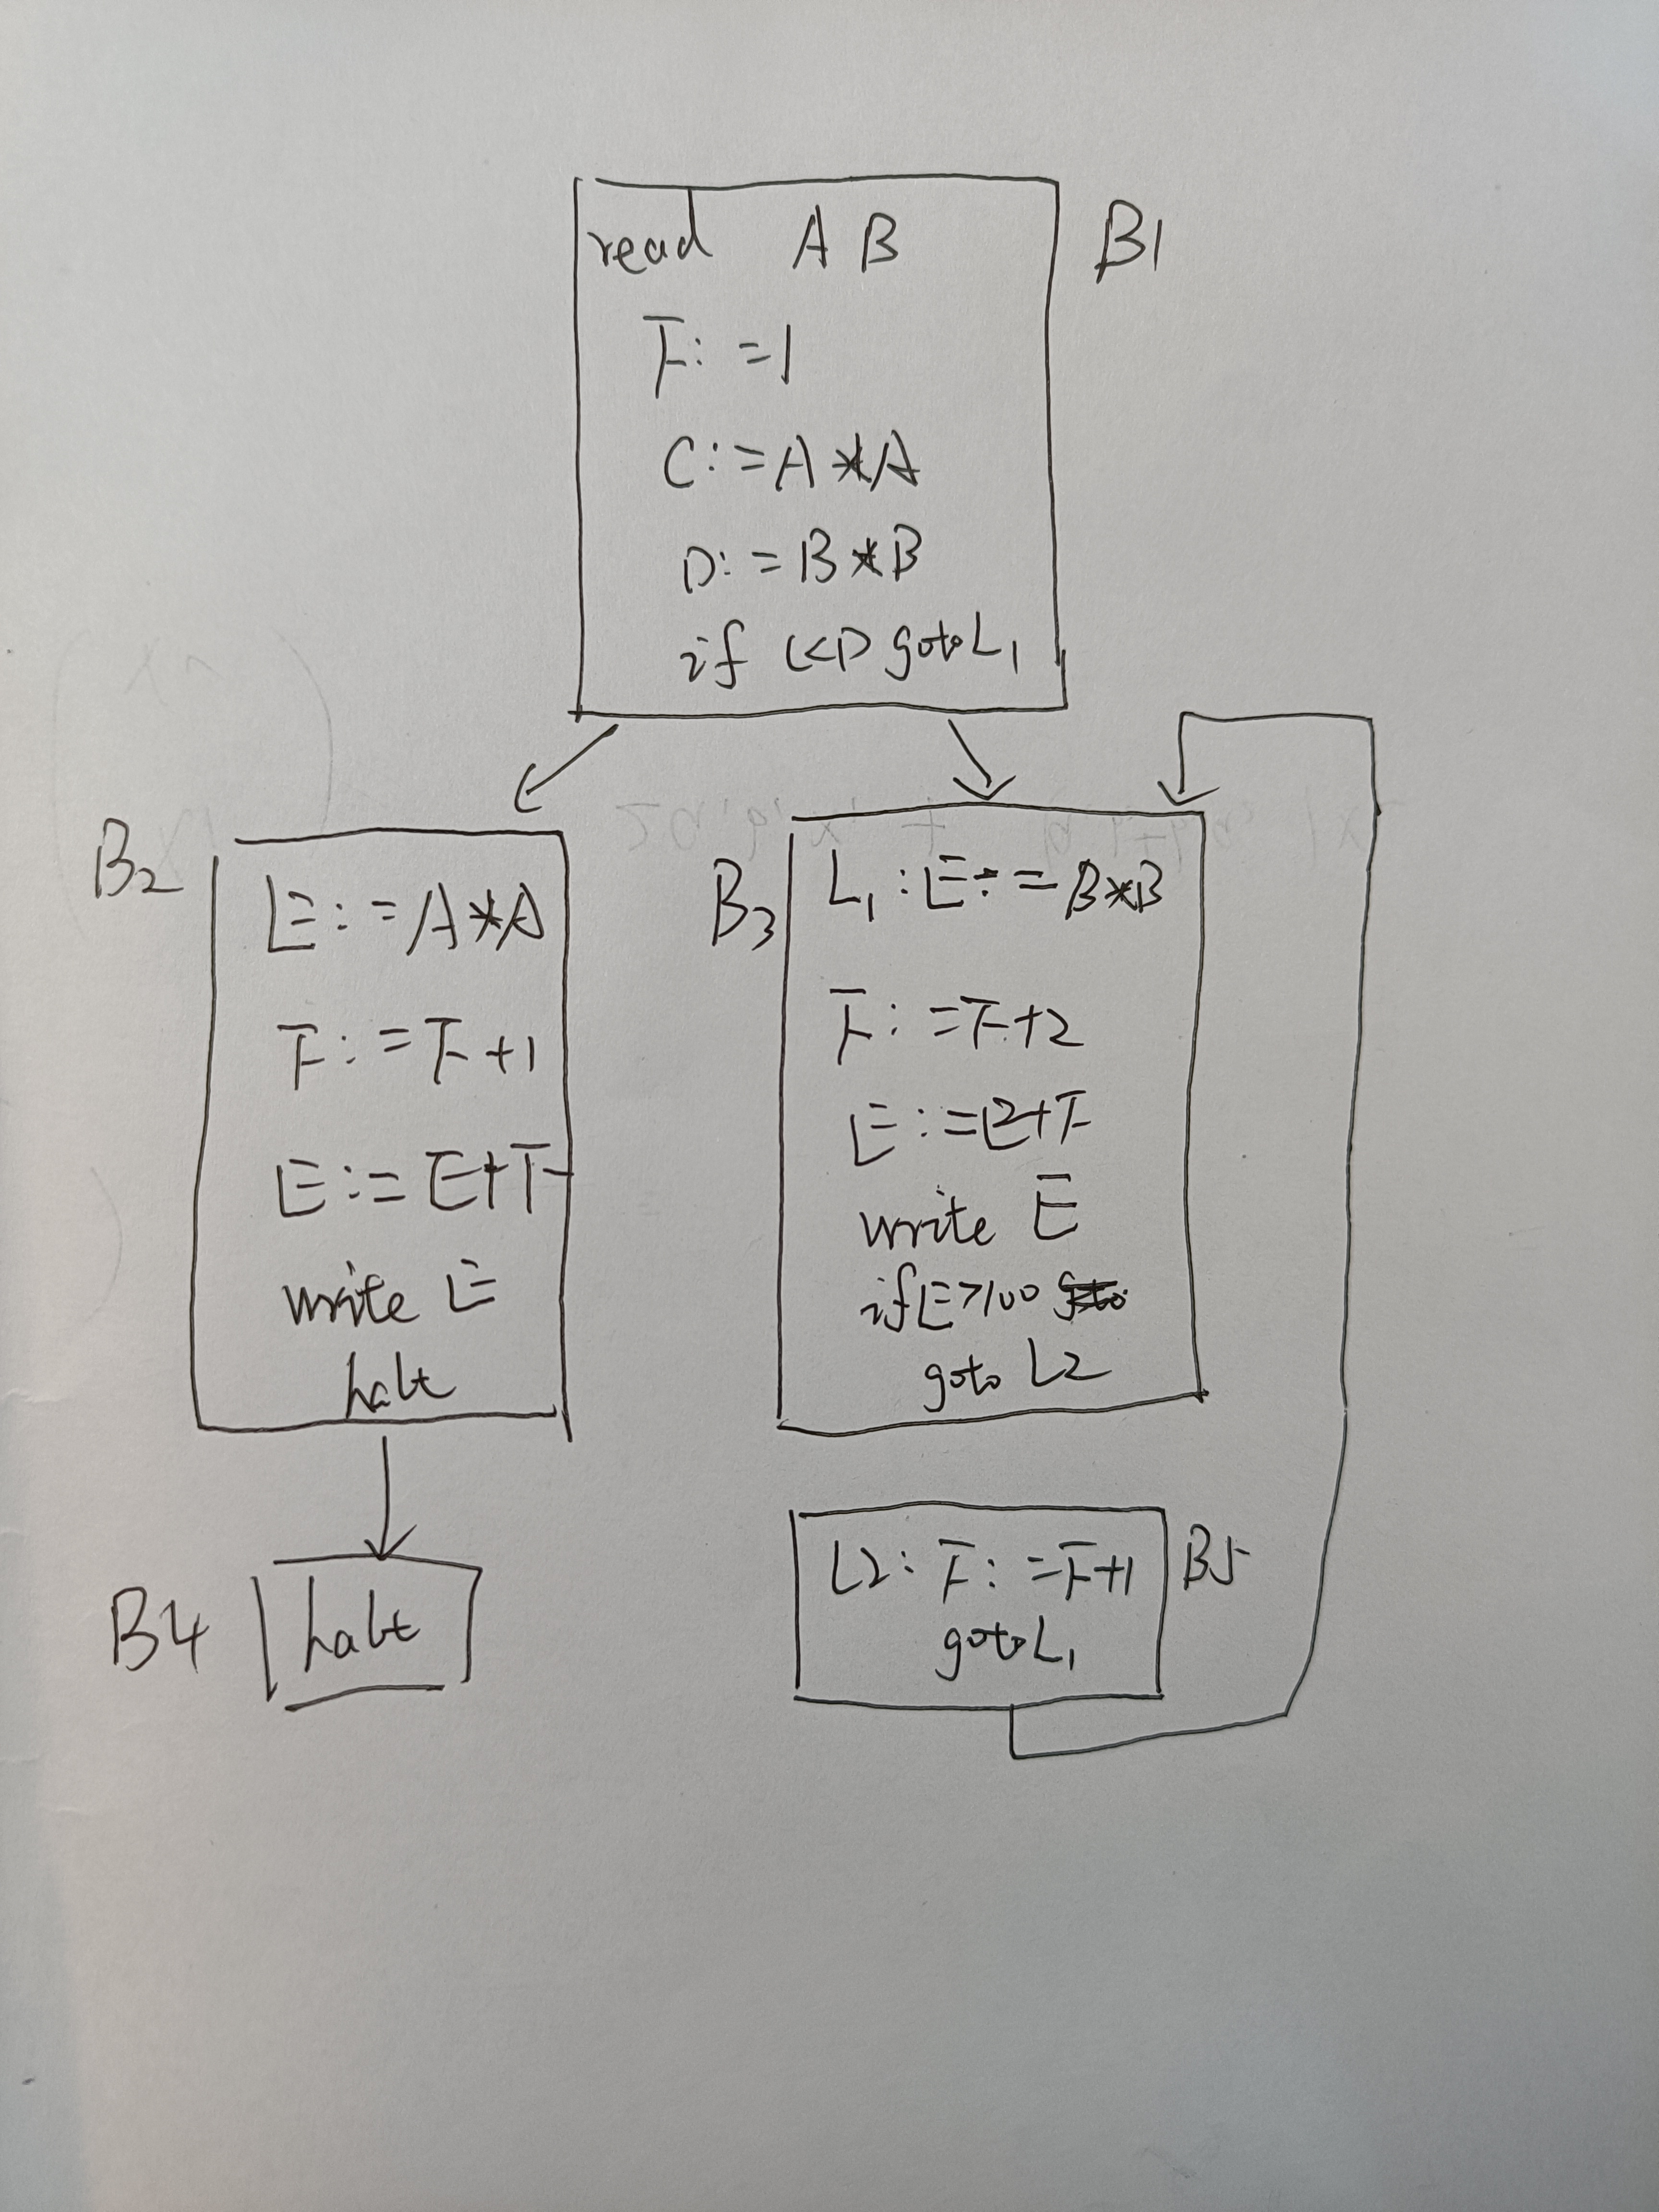
\includegraphics[height=16cm]{8_1.jpg}

\textbf{10.3.}

\begin{verbatim}
    B1:
    (1) 
    G := B*C
    S1 := G*G
    L := S1*G
    M := L

    (2) S1 := B*C
    S2 := S1*S1L := S2*S1

    B2:
    (1) 
    G := 3*F
    S1 := A+C
    S2 := A*C
    S3 := S1+S2
    L := 15+S3

    (2) S1 := A+C
    S2 := A*C
    S3 := S1+S2
    L := 15+S3
\end{verbatim}
\end{document}